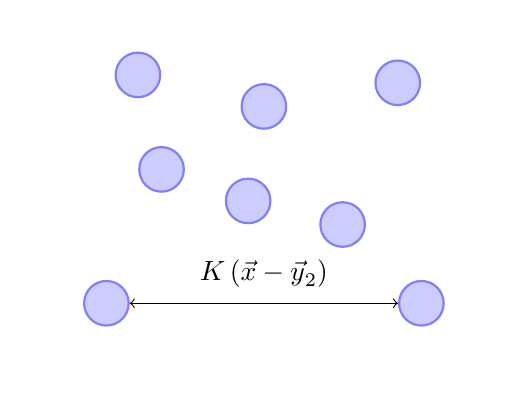
\begin{tikzpicture}[
    inner sep=2mm,
    particle/.style={circle, draw=blue!50, fill=blue!20, thick},
  ]
  \node [particle] (a) at (0, 0) {};
  \node [particle] (b) at (4, 0) {};
  \node [particle] at (2, 2.5) {};
  \node [particle] at (1.8, 1.3) {};
  \node [particle] at (0.7, 1.7) {};
  \node [particle] at (3, 1) {};
  \node [particle] at (3.7, 2.8) {};
  \node [particle] at (0.4, 2.9) {};
  \draw[<->] (a.east) -- (b.west) node [midway, above] {$K\left(\norm{\vec{x} - \vec{y}}_2\right)$};

  \useasboundingbox (-1,-1) rectangle (5, 3.5);
  % \draw [thick] (current bounding box.north east) -- (current bounding box.north west) -- (current bounding box.south west) -- (current bounding box.south east) -- cycle;
  % \node [anchor=south west, gray] at (-1.1, -1.1) {Bounding Box $\Omega$};
\end{tikzpicture}
